\documentclass[journal, a4paper]{IEEEtran}

% some very useful LaTeX packages include:

%\usepackage{cite}      % Written by Donald Arseneau
                        % V1.6 and later of IEEEtran pre-defines the format
                        % of the cite.sty package \cite{} output to follow
                        % that of IEEE. Loading the cite package will
                        % result in citation numbers being automatically
                        % sorted and properly "ranged". i.e.,
                        % [1], [9], [2], [7], [5], [6]
                        % (without using cite.sty)
                        % will become:
                        % [1], [2], [5]--[7], [9] (using cite.sty)
                        % cite.sty's \cite will automatically add leading
                        % space, if needed. Use cite.sty's noadjust option
                        % (cite.sty V3.8 and later) if you want to turn this
                        % off. cite.sty is already installed on most LaTeX
                        % systems. The latest version can be obtained at:
                        % http://www.ctan.org/tex-archive/macros/latex/contrib/supported/cite/

\usepackage{graphicx}   % Written by David Carlisle and Sebastian Rahtz
                        % Required if you want graphics, photos, etc.
                        % graphicx.sty is already installed on most LaTeX
                        % systems. The latest version and documentation can
                        % be obtained at:
                        % http://www.ctan.org/tex-archive/macros/latex/required/graphics/
                        % Another good source of documentation is "Using
                        % Imported Graphics in LaTeX2e" by Keith Reckdahl
                        % which can be found as esplatex.ps and epslatex.pdf
                        % at: http://www.ctan.org/tex-archive/info/

%\usepackage{psfrag}    % Written by Craig Barratt, Michael C. Grant,
                        % and David Carlisle
                        % This package allows you to substitute LaTeX
                        % commands for text in imported EPS graphic files.
                        % In this way, LaTeX symbols can be placed into
                        % graphics that have been generated by other
                        % applications. You must use latex->dvips->ps2pdf
                        % workflow (not direct pdf output from pdflatex) if
                        % you wish to use this capability because it works
                        % via some PostScript tricks. Alternatively, the
                        % graphics could be processed as separate files via
                        % psfrag and dvips, then converted to PDF for
                        % inclusion in the main file which uses pdflatex.
                        % Docs are in "The PSfrag System" by Michael C. Grant
                        % and David Carlisle. There is also some information
                        % about using psfrag in "Using Imported Graphics in
                        % LaTeX2e" by Keith Reckdahl which documents the
                        % graphicx package (see above). The psfrag package
                        % and documentation can be obtained at:
                        % http://www.ctan.org/tex-archive/macros/latex/contrib/supported/psfrag/

%\usepackage{subfigure} % Written by Steven Douglas Cochran
                        % This package makes it easy to put subfigures
                        % in your figures. i.e., "figure 1a and 1b"
                        % Docs are in "Using Imported Graphics in LaTeX2e"
                        % by Keith Reckdahl which also documents the graphicx
                        % package (see above). subfigure.sty is already
                        % installed on most LaTeX systems. The latest version
                        % and documentation can be obtained at:
                        % http://www.ctan.org/tex-archive/macros/latex/contrib/supported/subfigure/

\usepackage{url}        % Written by Donald Arseneau
                        % Provides better support for handling and breaking
                        % URLs. url.sty is already installed on most LaTeX
                        % systems. The latest version can be obtained at:
                        % http://www.ctan.org/tex-archive/macros/latex/contrib/other/misc/
                        % Read the url.sty source comments for usage information.

%\usepackage{stfloats}  % Written by Sigitas Tolusis
                        % Gives LaTeX2e the ability to do double column
                        % floats at the bottom of the page as well as the top.
                        % (e.g., "\begin{figure*}[!b]" is not normally
                        % possible in LaTeX2e). This is an invasive package
                        % which rewrites many portions of the LaTeX2e output
                        % routines. It may not work with other packages that
                        % modify the LaTeX2e output routine and/or with other
                        % versions of LaTeX. The latest version and
                        % documentation can be obtained at:
                        % http://www.ctan.org/tex-archive/macros/latex/contrib/supported/sttools/
                        % Documentation is contained in the stfloats.sty
                        % comments as well as in the presfull.pdf file.
                        % Do not use the stfloats baselinefloat ability as
                        % IEEE does not allow \baselineskip to stretch.
                        % Authors submitting work to the IEEE should note
                        % that IEEE rarely uses double column equations and
                        % that authors should try to avoid such use.
                        % Do not be tempted to use the cuted.sty or
                        % midfloat.sty package (by the same author) as IEEE
                        % does not format its papers in such ways.

\usepackage{amsmath}    % From the American Mathematical Society
                        % A popular package that provides many helpful commands
                        % for dealing with mathematics. Note that the AMSmath
                        % package sets \interdisplaylinepenalty to 10000 thus
                        % preventing page breaks from occurring within multiline
                        % equations. Use:
%\interdisplaylinepenalty=2500
                        % after loading amsmath to restore such page breaks
                        % as IEEEtran.cls normally does. amsmath.sty is already
                        % installed on most LaTeX systems. The latest version
                        % and documentation can be obtained at:
                        % http://www.ctan.org/tex-archive/macros/latex/required/amslatex/math/


\usepackage{amssymb}
\usepackage{mathtools}
\usepackage{physics}
\usepackage{float}

% Other popular packages for formatting tables and equations include:

%\usepackage{array}
% Frank Mittelbach's and David Carlisle's array.sty which improves the
% LaTeX2e array and tabular environments to provide better appearances and
% additional user controls. array.sty is already installed on most systems.
% The latest version and documentation can be obtained at:
% http://www.ctan.org/tex-archive/macros/latex/required/tools/

% V1.6 of IEEEtran contains the IEEEeqnarray family of commands that can
% be used to generate multiline equations as well as matrices, tables, etc.

% Also of notable interest:
% Scott Pakin's eqparbox package for creating (automatically sized) equal
% width boxes. Available:
% http://www.ctan.org/tex-archive/macros/latex/contrib/supported/eqparbox/

% *** Do not adjust lengths that control margins, column widths, etc. ***
% *** Do not use packages that alter fonts (such as pslatex).         ***
% There should be no need to do such things with IEEEtran.cls V1.6 and later.


% Your document starts here!
\begin{document}

% Define document title and author
	\title{Towards developing a streptobacillus model of bacteria based cell models implemented in Chaste}
	\author{Jonathan Miller
	\thanks{Advisor: Dr. Phillip Murray}}
	\markboth{Mathematical Biology: alignment and attractive ends forces}{}
	\maketitle

% Write abstract here
\begin{abstract}
	 Bacilli is the name given to any bacteria shaped like a rod. Chaste (Cancer, Heart and Soft Tissue Environment) has accommodated bacilli bacteria populations by developing an intersecting spheres model to maintain the rod like shape of bacteria during interaction. This \textbf{capsule force} is designed to ensure no capsule overlaps another capsule. As is known Streptobacilli is the name given to bacilli arranged in a chain. Chaste had not developed models to accommodate such chains.
\end{abstract}

% Each section begins with a \section{title} command
\section{Introduction}
	% \PARstart{}{} creates a tall first letter for this first paragraph
	\PARstart{F}{orces} are implemented in Chaste to aid in the understanding of natural phenomena. These forces are developed for simulation advantages, so as to visualise experimental results of questions posed by researchers in various area of study. Chaste can currently visualise up to three dimensions of simulations with \textit{cell-centre} and vertex \textit{vertex-based} cell populations. It can define different force laws for cell to cell interaction, different cell cycles, different cell proliferative types, to say a few \cite{ChasteCell}. Using an \textit{agile} approach to software development, Chaste develops new projects in directive intense bursts of code development, followed up by refactoring. In a recent code development burst, bacilli shaped cells were developed into working forces of cell cell interactions. This \textbf{capsule force}, $F_c$, operates when two capsules have overlapped by some distance $d$. A repulsive force is applied to the location of any and all capsules with a $d > 0$, meaning the capsules are overlapping by $d$. This $F_c$ only ensure no two capsules will overlap, it does nothing to affecting the topology of the population, namely developing force laws that do two tasks:
	\begin{enumerate}
	    \item Adhesion of capsules at their end points
	    \item Alignment of capsules with angles, $\theta_i < \frac{\pi}{2}$, between any two neighboring capsules, for $i\in P$, $P$ being the population of cells.
	\end{enumerate}
    This report will outline the progress of developing Chaste code to accommodate \textbf{(1)} and \textbf{(2)}. Furthermore, this report will detail visuals relating to development of code. 
% Main Part
\section{Bacterial Capsules and Capsule Force}
	Consider a bacterial capsule to be the construction of a cylinder and two hemispheres, such that a capsule is formed in $\mathbb{R}^n$. Let each capsule be $C_i$ and the determining attributes be a length $l_i$ and a radius $r_i$, such that $C_i = l_i+r_i$. This capsule is abstracted to a a problem of sliding spheres on rods and hence is a matter of intersecting spheres. When two capsules interact, say $C_i$ and $C_j$, there is said to be an \textbf{adhesive force} if each capsule, at its end points touches. If this criterion is met, then the capsules will adhere to each other. If the angle, $\theta$, that is the angle found to be between the two capsules, is $\frac{\pi}{2} \leq \theta \leq \pi $, then an \textbf{alignment force} will be applied to each capsule so that over time, the capsules will converge to $\theta = \pi$.
	\begin{figure}[H]
	    \centering
	    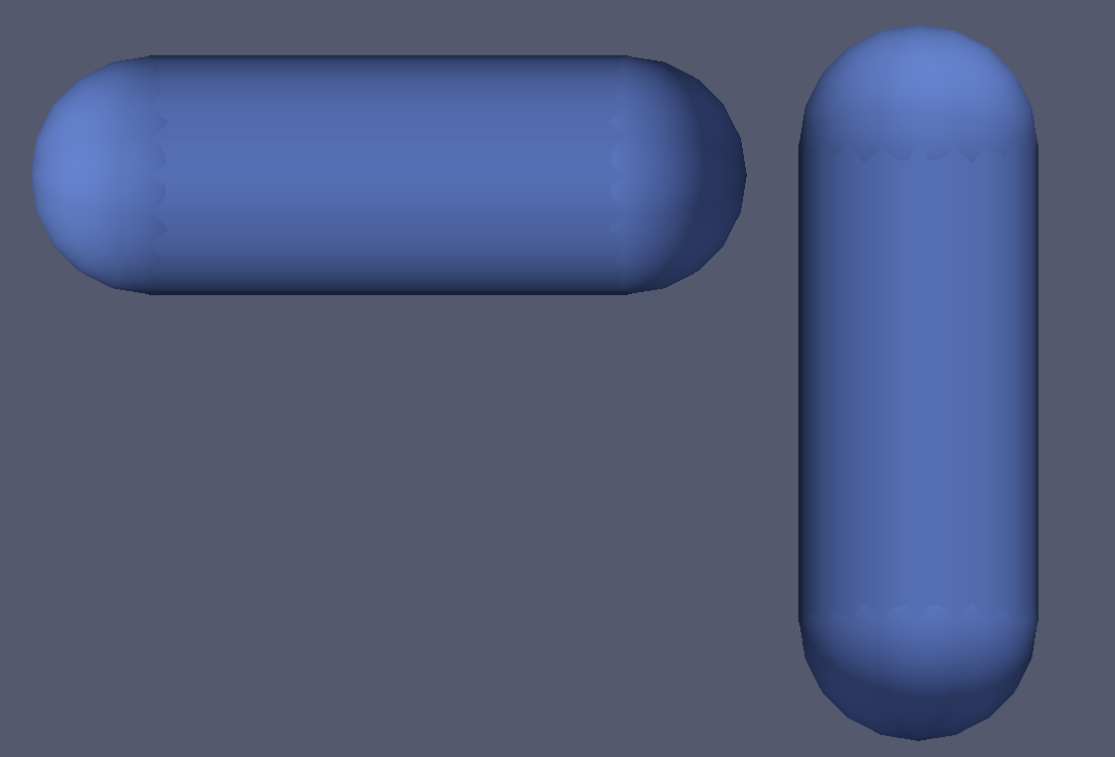
\includegraphics[scale = 0.22]{TwoCapsules.png}
	    \caption{Rod shaped capsules visualised in ParaView}
	    \label{fig:two_capsules}
	\end{figure}
		\begin{figure}[H]
	    \centering
	    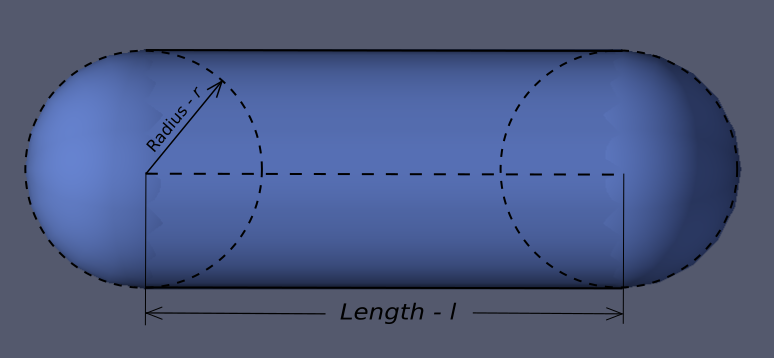
\includegraphics[scale = 0.32]{AnatomyOfCapsules.png}
	    \caption{Anatomy of a capsule}
	    \label{fig:anatomy_capsules}
	\end{figure}
	Consider that a capsule is considered to be the sum of a tube and two hemispheres, then for capsule \textbf{a}, say $C_a$ is $C_a=2r_a+l_a$. Then this model of capsules can be reduced to models of intersecting spheres. Suppose then, that two capsules overlap.
	\begin{figure}[H]
	    \centering
	    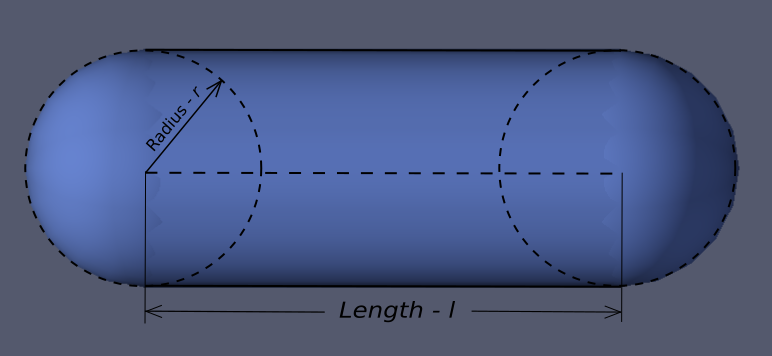
\includegraphics[scale = 0.22]{OverlappingCapsules.png}
	    \caption{Two capsules overlapping}
	    \label{fig:overlapping_capsules}
	\end{figure}
	Figure 3 shows two overlapping capsules. The overlapping dotted circles are re-visuluaised as shown below.
	\begin{figure}[H]
	    \centering
	    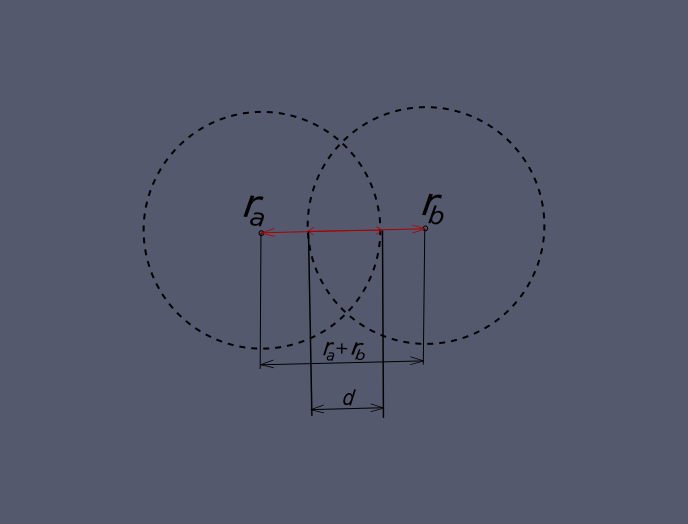
\includegraphics[scale = 0.42]{SkeletonOverlap.png}
	    \caption{Labelled overlap}
	    \label{fig:skeleton_overlap}
	\end{figure}	
    Two capsules overlapping are said to have an overlap, $d>0$ and two capsules that are neighbors and not overlapping have $d<0$. Under the $F_c$(\textbf{capsule force}), these two capsules' locations will be mutually repelled until $d=0$. 
\section{Forces}

\subsubsection{Capsules}
\subsubsection{Adhesive ends}
\subsubsection{Alignment}
There are four cases to consider.
\begin{enumerate}
    \item Two dimensional alignment
    \item Two dimensional alignment and anti-alignment
    \item Three dimensional alignment
    \item Three dimensional alignment and anti-alignment
\end{enumerate}
\begin{align}
    E   & = -\gamma (t_1\cdot t_2) \\
    F   & = -\nabla E \\
        & = -\gamma \left(\pdv{E}{\theta_1},\pdv{E}{\theta_2}\right)
\end{align}
Such that we seek to find the minimum of $E$.
\section{Methodology}
\section{Results}
\section{Conclusion}
% Now we need a bibliography:
\begin{thebibliography}{5}

	%Each item starts with a \bibitem{reference} command and the details thereafter.
	\bibitem{ChasteCell}
	Chaste (Cancer, Heart and Soft Tissue Environment) Cell-based Chaste: a multiscale computational framework for modelling cell populations
	\url{http://www.cs.ox.ac.uk/chaste/cell_based_index.html}
	\bibitem{MJH06} % Conference paper
	T.~Mayer, H.~Jenkac, and J.~Hagenauer. Turbo base-station cooperation for intercell interference cancellation. {\em IEEE Int. Conf. Commun. (ICC)}, Istanbul, Turkey, pp.~356--361, June 2006.

	\bibitem{Proakis} % Book
	J.~G.~Proakis. {\em Digital Communications}. McGraw-Hill Book Co.,
	New York, USA, 3rd edition, 1995.

	\bibitem{talk} % Web document
	F.~R.~Kschischang. Giving a talk: Guidelines for the Preparation and Presentation of Technical Seminars.
	\url{http://www.comm.toronto.edu/frank/guide/guide.pdf}.

	\bibitem{5}
	IEEE Transactions \LaTeX and Microsoft Word Style Files.
	\url{http://www.ieee.org/web/publications/authors/transjnl/index.html}

\end{thebibliography}

% Your document ends here!
\end{document}